\begin{tiny}
\begin{equation} 
\label{eq:1} 
    \Lagr_{c}(x, x^+, x^-) = \sum_{x \in X} \max(0,\mathrel{\Vert} f(x) -  f(x^+) \mathrel{\Vert}_2^2 - \mathrel{\Vert} f(x) - f(x^-) \mathrel{\Vert}_2^2 + \epsilon)
\end{equation}\\
\begin{equation} 
\label{eq:2} 
    \Lagr_{a}(x) = \sum_{x \in X} \max(0,\mathrel{\Vert} f(x) - f_a(x) \mathrel{\Vert}_2^2 + \epsilon_{a})
\end{equation}
\begin{equation} 
\label{eq:3} 
    \Lagr_{r}(x^+, x^-) = \sum_{x \in X} \max(0,-y * (f(x^+)-f(-x) + \epsilon_{r})
\end{equation}
\begin{equation} \label{eq:4} 
    \Lagr_{CAPOT}(x, x^+, x^- ) = \sum_{x \in X} \tau_{c} * \Lagr_{c} 
    + \tau_{a} *  \Lagr_{a} + \tau_{r} * \Lagr_{r} 
\end{equation}
\end{tiny}
\subsection{Motivation}
A robust query encoder seeks to represent queries with a shared intent in a common latent space such that minor variations in the formulation of the intent lead to similar document ranking. Prior work has shown that data augmentation and typo-optimized models increase model robustness, but it is not without cost.\\
Data augmentation requires changes to existing training methodologies and complete regeneration of the passage index. Given that the generation of the passage index can take longer than it does to train the model \cite{Karpukhin2020DensePR} regenerating a new index and retraining a model every time a novel form of noise is discovered is not tractable. Optimized pre-trained models can provide effective modeling solutions. However, given the rapid iteration pace of pretrained language models, making typo-aware variants for each new advance is hard to scale.\\
Motivated to improve performance without altering the underlying pretrained model or the bi-encoder training regime, we introduce CAPOT, a new methodology for increasing model robustness which is \textbf{computationally inexpensive} and \textbf{independent of training}. CAPOT works well because it can focus on improving the query encoder and leverages the short nature of queries to scale to large batch sizes. 
\subsection{CAPOT}
\textbf{C}ontrastive \textbf{A}lligment \textbf{Po}st \textbf{T}raining (CAPOT) is an expansion on traditional contrastive learning focused on making dual encoders robust to noise. The goal of CAPOT is to allow representations of noisy queries to be close to their original on the traditional triplet contrastive loss \cite{Schroff2015FaceNetAU} in \ref{eq:1}, where $f$ is a query encoder, $x$ is the original query, $x^+$ is a query where noise has been introduced, and $x^-$ is a negative query selected at random \footnote{We explore the usage of hard negatives mined from nearby query representation but did not find any measurable impact}. We modify \ref{eq:1} to scale the role of positive and negative samples using term specific in$\tau_{positive}$ and $\tau_{negative}$\ parameters. \\
While \ref{eq:1} allows the query-encoder to represent queries and noisy queries in a similar latent space, it has the unwanted side effect of query representation drifting related to the learned notion of relevance. Without controlling for this drift, a complete collapse in ranking accuracy came at the expense of effective representation of noisy samples. To avoid this, we introduce an anchoring term,\ref{eq:2}, that minimizes the drift between learning a notion of relevance and shared embeddings for queries with noise where $f$ is the noise-robust query-encoder, and $f_a$ is a copy of the unaltered frozen query-encoder, optimized for an existing document encoder and document index. \\
Seeking to improve performance further, we add a ranking loss as shown in \ref{eq:3} between the anchored model $f_a$ and $f$ where the model learns that $f(x^+)$ always ranks higher than $f_a(x)$. While this loss component is not crucial, we can leverage this to improve model performance slightly. \ref{eq:1},\ref{eq:2} and \ref{eq:3} are combined to form the CAPOT, \ref{eq:4}. 
\subsection{Experimental Approach}
\label{sec:ea}
To qualify the effectiveness, we explore how alignment can improve performance on noisy queries before and after bi-encoder training and compare them to data augmentation. We then compare the performance of the aligned models with unaltered baselines and models trained with DA. Except for models aligned with CAPOT, each experiment requires a complete training run and index generation, which can be quite slow. Each experiment is performed across 5 seeds, and we use the same evaluation metrics previously discussed and report the mean performance over five seeds.   \\
To quantify the ability of post-training alignment, we take the converged baseline models and apply CAPOT 
to align the model on the training portion of the query set. Once aligned, a model is retrieved on the unaligned, fixed document index generated during our baseline experimentation. Since queries are short and batch sizes can be scaled easily, it's important to note how fast this is. A single 2080ti NVIDIA GPU using CAPOT takes under 60 minutes on the NQ dataset. \\ 
To explore if alignment can happen before training, we leverage the ORCAS \cite{craswell2020orcas} dataset to generate a corpus of 10 million queries. Using these queries, we create positive and negative noisy samples using the same noising approach discussed in \ref{sec:making-noise} making a dataset of 100 million queries called Noisy-ORCAS \footnote{https://huggingface.co/datasets/spacemanidol/CAPOT-queries}. Using these 100m queries, we align the representation of queries and their noisy counterparts using a BERT-base model optimized for masked-language modeling. Given the scale of this dataset, We train for a single epoch on the Noisy-ORCAS corpus using the $\tau_{positive}=1.0$,$\tau_{negative}=0.1$,and $\tau_{anchor}=1.0$ on 4 V100 GPUs with a batch size of 2048. Then, we leverage this optimized model to initialize our unaltered bi-encoder model's training procedure. Then, this model is trained on our datasets and evaluated similarly to the baseline.  We refer to models trained this way as(PT), and each usage of PT requires retraining and index regeneration. 
\subsection{Experimental Results}
\begin{figure}[!htb]
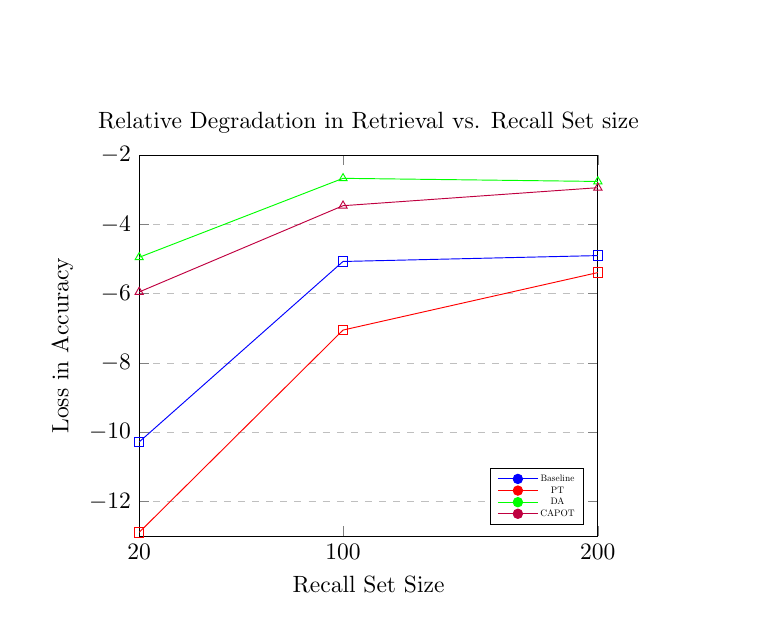
\begin{tikzpicture}
\scalebox{0.85}{
\begin{axis}[
    title={Relative Degradation in Retrieval  vs. Recall Set size},
    xlabel={Recall Set Size},
    ylabel={Loss in Accuracy},
    xmin=20, xmax=200,
    ymin=-13 , ymax=-2,
    xtick={20, 100, 200},
    ytick={-12,-10,-8,-6,-4,-2},
    legend pos=south east,
    ymajorgrids=true,
    grid style=dashed,
    legend style={nodes={scale=0.4, transform shape}}, 
    legend image post style={mark=*}
]
\addplot[
    color=blue,
    mark=square,
    ]
    coordinates {
    (20, -10.28) (100, -5.07 ) (200,-4.9 )
    };
\addplot[
    color=red,
    mark=square,
    ]
    coordinates {
    (20, -12.89) (100, -7.05 ) (200, -5.39)
    };
\addplot[
    color=green,
    mark=triangle,
    ]
    coordinates {
    (20, -4.95) (100, -2.67 ) (200, -2.76 )
    };
    
\addplot[
    color=purple,
    mark=triangle,
    ]
    coordinates {
    (20, -5.95) (100, -3.46 )(200,-2.94 )
    };
\legend{Baseline, PT, DA, CAPOT }
 \end{axis}}
\end{tikzpicture}
    \centering
    \caption{Average Relative loss in bi-encoder recall accuracy on NQ by recall set size depth on the baseline, Pretrained Alignment (PT), Data Augmentation (DA), and Contrastive Alignment Post Training (CAPOT) on noisy queries.}
    \label{fig:CAPOT-all-nq}
\end{figure}
As shown in figures \ref{fig:CAPOT-all-nq} and \ref{fig:CAPOT-typo-nq}, using CAPOT can improve performance on queries with noise, particularly typos. Moreover, the impact of CAPOT is similar to DA without a training set alteration or index regeneration. CAPOT approach takes advantage of training on only the query encoder and fixing the document encoder. Since queries tend to be short, CAPOT uses a max sequence length of 28 tokens to minimize memory usage, allowing scaling to batch sizes of 2048 on GPUs with 16 GBs. This large batch size means training is rapid and effective. A complete alignment run on the NQ dataset takes one hour on a single V100 gpu. At the same time, data augmentation requires 26 hours for training and an additional day for index generation (50 hours overall).\\ 
\begin{figure}[!htb]
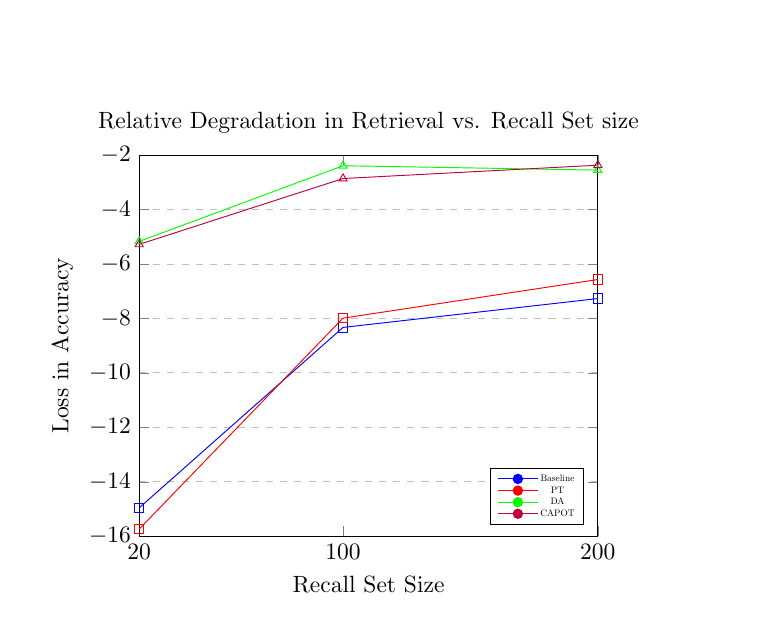
\begin{tikzpicture}
\scalebox{0.85}{
\begin{axis}[
    title={Relative Degradation in Retrieval  vs. Recall Set size},
    xlabel={Recall Set Size},
    ylabel={Loss in Accuracy},
    xmin=20, xmax=200,
    ymin=-16 , ymax=-2,
    xtick={20, 100, 200},
    ytick={-16,-14,-12,-10,-8,-6,-4,-2},
    legend pos=south east,
    ymajorgrids=true,
    grid style=dashed,
    legend style={nodes={scale=0.4, transform shape}}, 
    legend image post style={mark=*}
]
\addplot[
    color=blue,
    mark=square,
    ]
    coordinates {
    (20, -14.96) (100, -8.33) (200,-7.27 )
    };
\addplot[
    color=red,
    mark=square,
    ]
    coordinates {
    (20, -15.74) (100, -7.99 ) (200, -6.57)
    };
\addplot[
    color=green,
    mark=triangle,
    ]
    coordinates {
    (20, -5.17) (100, -2.39 ) (200, -2.55 )
    };
    
\addplot[
    color=purple,
    mark=triangle,
    ]
    coordinates {
    (20, -5.28) (100, -2.86 )(200,-2.37 )
    };
\legend{Baseline, PT, DA, CAPOT }
 \end{axis}}
\end{tikzpicture}
    \centering
    \caption{Average Relative loss in bi-encoder recall accuracy on NQ by recall set size depth on the baseline, Pretrained Alignment (PT), Data Augmentation (DA), and Contrastive Alignment Post Training (CAPOT) on character-based noisy queries (typos).}
    \label{fig:CAPOT-typo-nq}
\end{figure} 

\begin{table*}[!ht]
    \centering
    \tiny
    \begin{tabular}{|l|l|l|l|l|l|l|l|l|l|l|l|l|}
    \hline
    Dataset & \multicolumn{3}{l}{Regular} &  \multicolumn{3}{l}{DA} & \multicolumn{3}{l}{PT} & \multicolumn{3}{l}{CAPOT}  \\ \hline 
        Depth & 20 & 100 & 200 & 20 & 100 & 200 & 20 & 100 & 200 & 20 & 100 & 200 \\ \hline
        NQ & -10.28\% & -5.07\% & -4.91\% & -4.95\% & -2.67\% & -2.76\% & -12.89\% & -7.05\% & -5.39\% & -5.95\% & -3.46\% & -2.94\% \\ \hline
        TriviaQA & -4.90\% & -2.98\% & -2.24\% & -7.20\% & -4.44\% & -3.57\% & -11.89\% & -6.83\% & -5.34\% & -3.37\% & -1.68\% & -1.17\% \\ \hline
        MSMARCO  & -20.92\% & -33.91\% & -30.46\% & -43.98\% & -28.89\% & -16.73\% & -46.28\% & -36.41\% & -28.69\% & -22.76\% &	-16.73\% & -14.48\% \\ \hline
    \end{tabular}
    \caption{Relative degradation in retrieval accuracy at 20,100,200 on NQ,TriviaQA, and MSMARCO. Retrieval accuracy and relative loss across types of noise for unaltered (Regular),  Data Augmentation (DA),Pre Training Alignment (PT), and Post Training Contrastive Alignment (CAPOT)}
    \label{tab:capot-vs-other-aggregate}
\end{table*}
\begin{table*}[!ht]
    \centering
    \tiny
    \begin{tabular}{|l|l|l|l|l|l|l|l|l|l|l|l|l|}
    \hline
    Dataset & \multicolumn{3}{l}{Regular} &  \multicolumn{3}{l}{DA} & \multicolumn{3}{l}{PT} & \multicolumn{3}{l}{CAPOT}  \\ \hline 
        Depth & 20 & 100 & 200 & 20 & 100 & 200 & 20 & 100 & 200 & 20 & 100 & 200 \\ \hline
        NQ & -14.96\% & -8.33\% & -7.27\% & -5.17\% & -2.39\% & -2.55\% & -15.74\% & -7.99\% & -6.57\% & -5.28\% & -2.86\% & -2.37\% \\ \hline
        TriviaQA & -8.43\% & -4.56\% & -3.39\% & -7.71\% & -4.44\% & -3.64\% & -14.64\% & -8.28\% & -5.47\% & -3.39\% & -1.42\% & -0.87\% \\ \hline
        MSMARCO  & -41.68\% & -33.91\% & -30.46\% & -43.98\% & -33.70\% & -28.69\% & -55.58\% & -45.47\% & -40.95\% & -24.58\% & -18.40\% & -15.95\% \\ \hline
    \end{tabular}
    \caption{Relative degradation in retrieval accuracy at 20,100,200 on NQ,TriviaQA, and MSMARCO. Retrieval accuracy and relative loss across types of character alteration noise (typos) for unaltered (Regular),  Data Augmentation (DA),Pre Training Alignment (PT), and Post Training Contrastive Alignment (CAPOT)}
    \label{tab:capot-vs-other-aggregate-typo}
\end{table*}
Looking at summary metrics in table \ref{tab:capot-vs-other-aggregate} and \ref{tab:capot-vs-other-aggregate-typo}, we can see that the use of pre-training alignment is never optimal and always under-performs un unaltered network. We believe this indicates the importance of introducing noise after training. If introduced prior, the noise will likely be forgotten, and it will hamper the ability to learn a proper, relevant representation. \\

\section{Expanding Contrastive Alignment}
Seeking to explore the impact of variations in alignment query distribution's role, we explore how well CAPOT works with an alignment dataset that differs from the evaluation. To do so, we explore the impact of using the previously discussed Noisy-ORCAS dataset to align noisy queries for TriviaQA. Given the differences in dataset size, we train for the same number of optimization steps with the Noisy-Orcas data as we do with the regular data. \\
\begin{figure}[!htb]
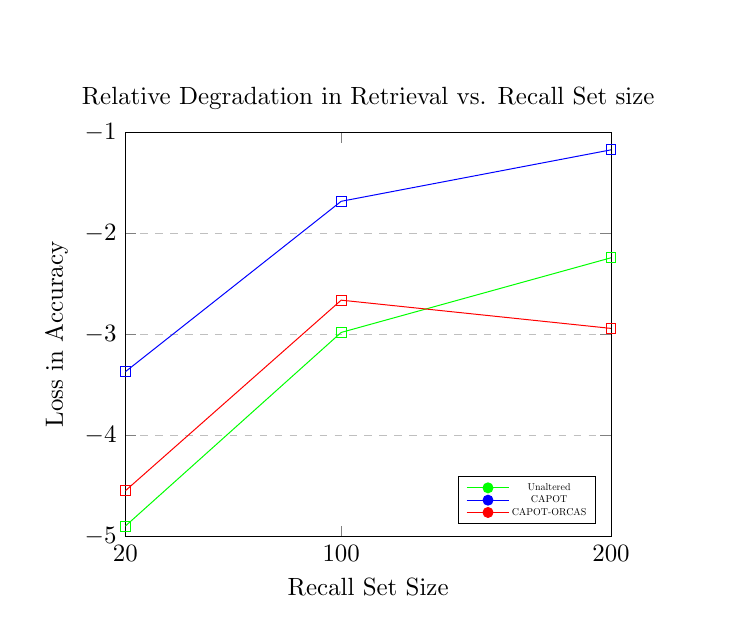
\begin{tikzpicture}
\scalebox{0.9}{
\begin{axis}[
    title={Relative Degradation in Retrieval  vs. Recall Set size},
    xlabel={Recall Set Size},
    ylabel={Loss in Accuracy},
    xmin=20, xmax=200,
    ymin=-5 , ymax=-1,
    xtick={20, 100, 200},
    ytick={-5,-4,-3,-2,-1},
    legend pos=south east,
    ymajorgrids=true,
    grid style=dashed,
    legend style={nodes={scale=0.4, transform shape}}, 
    legend image post style={mark=*}
]
\addplot[
    color=green,
    mark=square,
    ]
    coordinates {
    (20, -4.9) (100, -2.98) (200,-2.24 )
    };
\addplot[
    color=blue,
    mark=square,
    ]
    coordinates {
    (20, -3.37) (100, -1.68) (200,-1.17 )
    };
\addplot[
    color=red,
    mark=square,
    ]
    coordinates {
    (20, -4.55) (100, -2.66 ) (200, -2.94)
    };
\legend{Unaltered, CAPOT, CAPOT-ORCAS }
 \end{axis}}
\end{tikzpicture}
    \centering
    \caption{Average Relative loss in bi-encoder recall accuracy on NQ by recall set size depth on of unaltered,Contrastive Alignment Post Training (CAPOT) and Contrastive Alignment Post Training (CAPOT) ORCAS on TriviaQA.}
    \label{fig:CAPOT-orcas}
\end{figure} 
As shown in figure \ref{fig:CAPOT-orcas}, using an unrelated dataset, ORCAS, provides a close approximation to using the true query distribution, but it does not always outperform the un-altered baseline, indicated by the performance at 200. We believe this is expected as the true query distribution is a factor in how the query vector manifold is optimized.  